\documentclass[conference]{IEEEtran}

\usepackage{cite}
\usepackage{amsmath,amssymb}
\usepackage{graphicx}
\usepackage{booktabs}
\usepackage{multirow}
\usepackage{xcolor}
\usepackage{tikz}
\usetikzlibrary{positioning,arrows.meta,fit,calc}
\usepackage{pgfplots}
\pgfplotsset{compat=1.18}
\usepackage{url}
\usepackage[hidelinks]{hyperref}
\usepackage[capitalise]{cleveref}
\usepackage{placeins}

% Marks text the authors must fill in. Remove before submission.
\newcommand{\authornote}[1]{\textbf{\textcolor{blue}{[#1]}}}
\newcommand{\ns}{\textsuperscript{n.s.}}

\begin{document}

\title{Distilling a Chest X-ray Foundation Model Ensemble into a Lightweight CNN}

\author{
\IEEEauthorblockN{Tabassum Sumaiya, Md.\ Hasibul Hossain, Marjia Islam, Ashraful Islam Tanzil}
\IEEEauthorblockA{Department of Computer Science and Engineering, United International University\\
Dhaka, Bangladesh\\
}
}

\maketitle

% =====================================================================
\begin{abstract}
Chest X-ray foundation models reach strong accuracy on multi-label classification, but their inference cost limits deployment in high-throughput and resource-constrained settings We investigate whether knowledge distillation can transfer the performance of a foundation-model ensemble to a lightweight convolutional network. We construct a teacher ensemble by averaging calibrated predictions from ConvNeXt-Tiny, a convolutional neural network, and RAD-DINO, a chest X-ray foundation model based on a vision transformer. The ensemble is distilled into a new ConvNeXt-Tiny using a combination of ground-truth labels and teacher soft target.  On the official NIH ChestX-ray14 test set of 25,596 images from 2,797 patients, the distilled model achieves a macro AUROC of 0.8339, improving significantly over the independently trained CNN baseline (0.8263) and approaching RAD-DINO (0.8364). The distilled model retains the CNN's inference cost, requiring approximately 5.7$\times$ less compute than RAD-DINO at batch size 32. Improvements are observed across all 14 findings, although the remaining gap is larger for findings where higher-resolution inputs provide an advantage. These results show that distillation can transfer much of the predictive benefit of a foundation-model ensemble into a single lightweight CNN, providing a practical accuracy--efficiency trade-off for chest X-ray classification.
\end{abstract}


\begin{IEEEkeywords}
chest X-ray, knowledge distillation, foundation model, ensemble, efficient inference, multi-label classification.
\end{IEEEkeywords}

% =====================================================================
\section{Introduction}
\label{sec:intro}

The chest radiograph (chest X-ray, CXR) is the most commonly ordered imaging test for suspected lung disease~\cite{raoof2012interpretation}. In many health systems, the number of radiologists available to read these images has not kept pace with demand~\cite{rcr2025census}. Deep learning for automated CXR interpretation has therefore become a large research area~\cite{calli2021deep}. Public datasets such as NIH ChestX-ray14, with 112,120 frontal radiographs labelled for 14 findings~\cite{wang2017chestxray8}, made it possible to train CNNs for this task~\cite{rajpurkar2017chexnet}.

More recently, \emph{foundation models} have been built specifically for radiographs. These are large networks pretrained on broad data and then adapted to many tasks~\cite{moor2023foundation}. RAD-DINO is a Vision Transformer (ViT-B/14) pretrained on chest X-rays with the self-supervised DINOv2 method~\cite{perezgarcia2025raddino,oquab2024dinov2}. Its accuracy comes at a price. It has 86.6\,M parameters and reads $518\times518$ pixel inputs, which gives 1,369 image patches whose pairwise attention must be computed~\cite{dosovitskiy2021vit}. A modern CNN such as ConvNeXt-Tiny~\cite{liu2022convnext} has 27.8\,M parameters and works well at $384\times384$ pixels. On the GPU used in this study, RAD-DINO needed 22.8\,ms per image in batches of 32, against 4.0\,ms for ConvNeXt-Tiny.

Several approaches aim to keep a large model's accuracy at a lower cost. Cascades route inputs between a cheap and an expensive model at test time~\cite{wang2018idk,wang2022wisdom}, but they keep both models in deployment. Ensembles of different models are often more accurate than any single member~\cite{dietterich2000ensemble,lakshminarayanan2017deep}, but they multiply the cost. \emph{Knowledge distillation} (KD) avoids both problems. A small student is trained to reproduce the soft predictions of a stronger teacher, and only the student is run afterwards~\cite{bucilua2006model,hinton2015distilling,gou2021knowledge}. Its inference cost is fixed and equal to that of the student.

This paper combines the two ideas. We use the ensemble of a CNN and RAD-DINO as the teacher, and distil it into a single ConvNeXt-Tiny. Our contributions are:
\begin{enumerate}
  \item We show that ConvNeXt-Tiny and RAD-DINO are complementary on the official ChestX-ray14 test split: their calibrated average is significantly more accurate than either model alone.
  \item We distil this two-model teacher into one ConvNeXt-Tiny, trained with exactly the recipe of the original CNN. The distilled student is significantly more accurate than the CNN at the same cost, and it comes within 0.0025 macro AUROC of RAD-DINO at 5.7$\times$ lower batch cost. All decision rules were fixed before the experiment.
  \item We analyse per finding where the student gains, and how it recovers positives that only RAD-DINO had found.
\end{enumerate}

% =====================================================================
\section{Related Work}
\label{sec:related}

\subsection{Chest X-ray Classification and Foundation Models}
CNNs trained on ChestX-ray14, such as CheXNet~\cite{rajpurkar2017chexnet}, established the dataset as a standard benchmark~\cite{calli2021deep}. Its labels were mined from report text and contain errors~\cite{oakdenrayner2020exploring}. Models trained on one population can also perform worse on another~\cite{zech2018variable}, so results from different data splits are not directly comparable. Self-supervised foundation models trained on radiographs, such as RAD-DINO~\cite{perezgarcia2025raddino}, provide stronger starting features than networks pretrained on natural images~\cite{deng2009imagenet}, but their inference cost is rarely reported next to their accuracy.

\subsection{Ensembles}
Combining the predictions of several models usually improves accuracy, especially when the members make different errors~\cite{dietterich2000ensemble}. Averaging the outputs of independently trained deep networks is a simple and strong baseline~\cite{lakshminarayanan2017deep}. The price is that every member must be run on every input.

\subsection{Knowledge Distillation}
Distillation was introduced as model compression~\cite{bucilua2006model} and popularised with temperature-softened teacher outputs~\cite{hinton2015distilling}; a survey is given in~\cite{gou2021knowledge}. Distilling an ensemble into one network was one of the original motivations~\cite{bucilua2006model,hinton2015distilling}. Soft targets can also reduce the effect of noisy labels~\cite{li2017noisy}, and even a student with the same architecture as its teacher can improve on it~\cite{furlanello2018born}. Larger teachers do not always make better students~\cite{cho2019efficacy,mirzadeh2020teacher}. For CXRs, Ho and Gwak distilled larger CNNs into lightweight students on ChestX-ray14~\cite{ho2020utilizing}. Termritthikun et~al.\ compared CNN and transformer teachers for an on-device student~\cite{termritthikun2024explainable}, and Kishore et~al.\ distilled a self-supervised teacher into a compressed student~\cite{kishore2025enhancing}. We did not find a study that distils RAD-DINO, or an ensemble containing it, into a CNN.

% =====================================================================
\section{Methods}
\label{sec:methods}

\Cref{fig:pipeline} summarises the method: two trained models form a teacher ensemble, the ensemble labels the training images with soft probabilities, and a new CNN learns from these labels. Only the student runs at test time.

\begin{figure}[htbp]
\centering
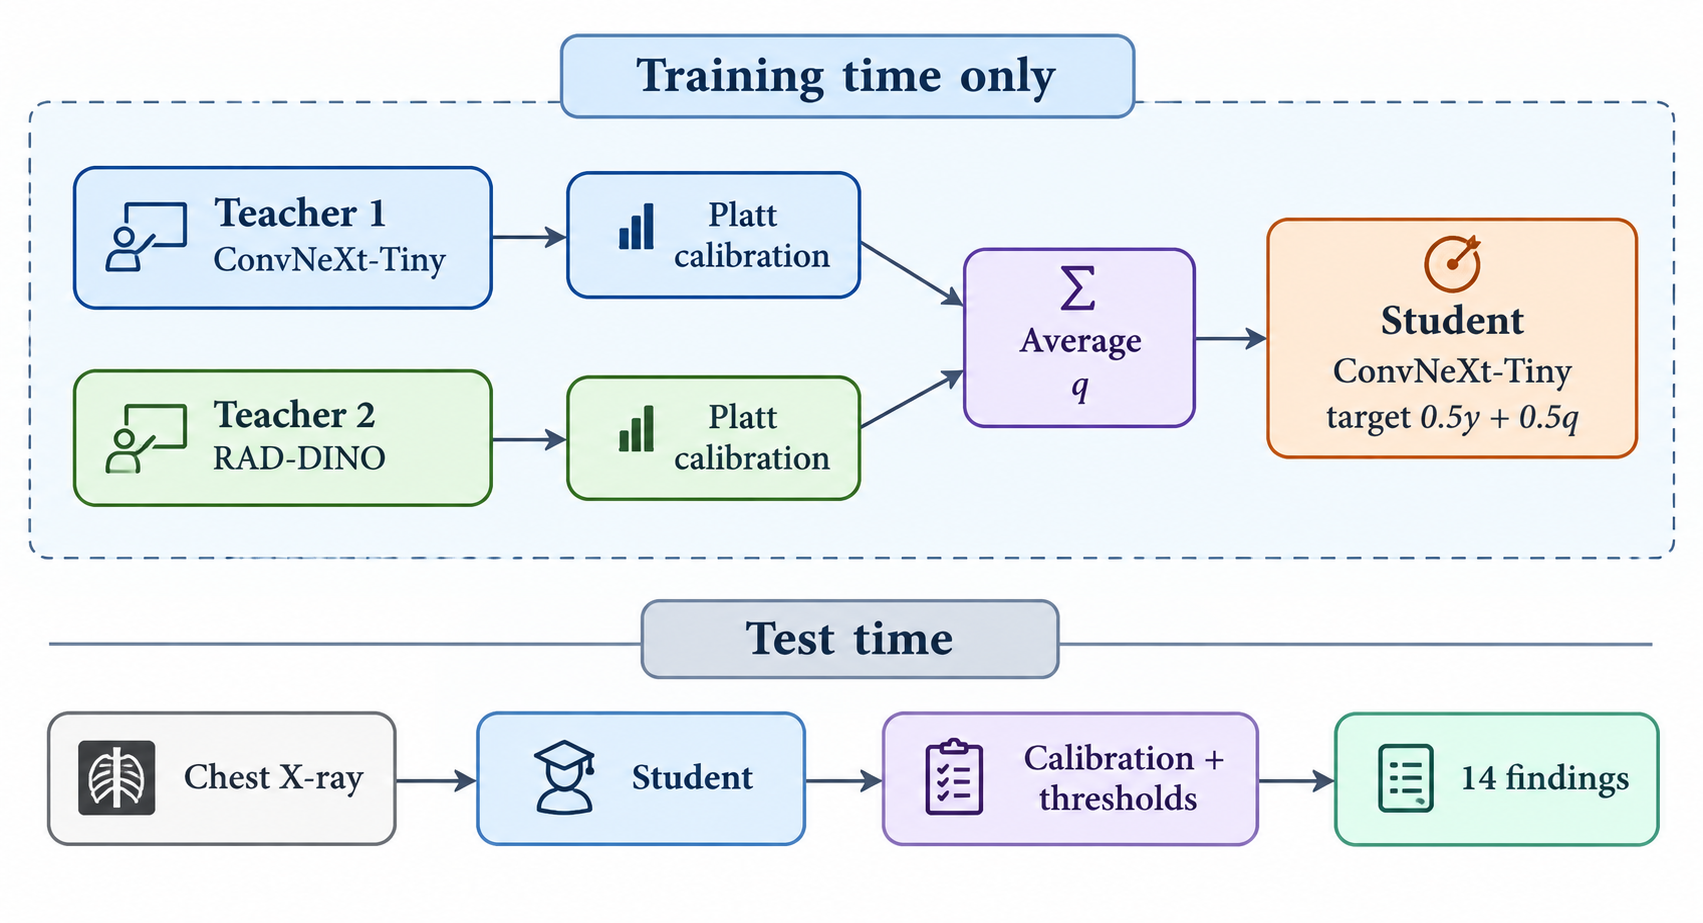
\includegraphics[width=\columnwidth]{figures/pipeline_diagram.png}
\caption{Distillation pipeline. The two calibrated teachers are averaged into soft labels $q$ for the training images. The student learns from $q$ and the real labels $y$. At test time only the student runs, at the cost of the original CNN.}
\label{fig:pipeline}
\end{figure}

\subsection{Data}
We use NIH ChestX-ray14~\cite{wang2017chestxray8}, which contains frontal radiographs labelled for 14 findings. The task is multi-label: an image can carry several findings, and an image with no finding has an all-zero label vector. The official test list is kept unchanged. A validation set is drawn from 15\% of the official train/validation \emph{patients}, so that no patient appears in more than one partition. The split is fixed by SHA-256 hashes that every experiment checks. \Cref{tab:data} shows that the official test population is harder than the development data. It has more findings per image and fewer standard posterior--anterior (PA) views.

\begin{table}[t]
\centering
\caption{Data partitions. The official test set carries more findings per image than the training and validation data.}
\label{tab:data}
\begin{tabular}{@{}lrrr@{}}
\toprule
 & Train & Validation & Test \\
\midrule
Images           & 73,916 & 12,608 & 25,596 \\
Patients         & 23,806 & 4,202  & 2,797 \\
Images per patient & 3.1 & 3.0 & 9.2 \\
Findings per image & 0.63 & 0.61 & 1.06 \\
Images with no finding & 58\% & 59\% & 39\% \\
PA views         & 65\% & 66\% & 43\% \\
\bottomrule
\end{tabular}
\end{table}

\subsection{Teacher Models}
\textbf{CNN.} ConvNeXt-Tiny~\cite{liu2022convnext}, pretrained on ImageNet-22k and fine-tuned on ImageNet-1k~\cite{deng2009imagenet}, with $384\times384$ input. The head consists of global average pooling, dropout 0.2 and a linear layer to 14 outputs. After one epoch that trains only the head, the whole network is fine-tuned for up to 8 epochs (learning rate $10^{-4}$, batch 32, stochastic depth 0.1).

\textbf{RAD-DINO.} ViT-B/14 from~\cite{perezgarcia2025raddino}, with $518\times518$ input. The CLS token is concatenated with the mean patch token and passed through dropout 0.2 and a linear layer. The model first trains only the head for 2 epochs. The last 8 of its 12 transformer blocks are then fine-tuned for up to 4 epochs with layer-wise learning-rate decay (0.8). The evaluated weights are an exponential moving average (decay 0.999).

\textbf{Shared recipe.} All networks, including the student, use the Asymmetric Loss (ASL)~\cite{ridnik2021asl} with $\gamma_+=1$, $\gamma_-=4$ and margin 0.05. This loss down-weights the many easy negatives of rare findings. Training uses AdamW with cosine decay, mixed precision and light augmentation (random resized crop, horizontal flip, $\pm7^\circ$ rotation, brightness/contrast jitter). Early stopping uses validation macro AUROC. Each model is trained once, with seed 42, on one NVIDIA Tesla T4.

\subsection{Calibration and Decision Thresholds}
For each finding $c$, the raw logit $z_c$ is turned into a probability with Platt scaling~\cite{platt1999probabilistic},
\begin{equation}
\hat{p}_c = \sigma(a_c z_c + b_c),
\label{eq:platt}
\end{equation}
where $a_c$ and $b_c$ are fitted on validation by minimising the negative log-likelihood. Calibration puts the two teachers on the same probability scale before they are averaged~\cite{guo2017calibration}. Each finding then gets its own yes/no threshold, chosen to maximise F1 on validation. All fitted values are applied unchanged to the test set.

\subsection{Teacher Ensemble}
The teacher is the equal-weight average of the two calibrated models:
\begin{equation}
q_{i,c} = \tfrac{1}{2}\left(\hat{p}^{\,\text{CNN}}_{i,c} + \hat{p}^{\,\text{RAD-DINO}}_{i,c}\right).
\label{eq:teacher}
\end{equation}
The equal weights were fixed in advance. The same average is also evaluated as a system of its own (``Average''), which shows how accurate the teacher is.

\subsection{Knowledge Distillation}
\textbf{Soft labels.} $q$ is computed once for the 73,916 training images, without augmentation. Validation and test images never receive soft labels.

\textbf{Go/no-go check.} The teachers were trained on the same images, so their soft labels might simply copy the real labels. We fixed in advance that the student would be trained only if the teacher's macro AUROC on the training images was below 0.95.

\textbf{Student.} The student is a new ConvNeXt-Tiny, initialised from ImageNet (not from the trained CNN) and trained with exactly the recipe of the original CNN. Only the training target changes:
\begin{equation}
t_{i,c} = (1-\lambda)\,y_{i,c} + \lambda\,q_{i,c}, \qquad \lambda = 0.5 .
\label{eq:target}
\end{equation}
Because ASL is linear in its target, this is equal to averaging the loss against the real label $y$ and the loss against the teacher $q$. Any difference between the student and the original CNN therefore comes from the teacher alone. At test time the student is followed by its own calibration~\eqref{eq:platt} and thresholds.

\subsection{Evaluation}
\textbf{Metrics.} The primary metric is macro AUROC, the mean over the 14 findings of the area under the ROC curve~\cite{hanley1982meaning}. Secondary metrics are macro AUPRC, macro and micro F1, and recall and precision at the fitted thresholds.

\textbf{Uncertainty.} 95\% confidence intervals come from 1,000 bootstrap resamples of test \emph{patients}~\cite{efron1993bootstrap}. Resampling patients matters because test patients have 9.2 images on average. Systems are compared on the same resamples. A difference is called significant only if its CI excludes zero \emph{and} its Holm-corrected~\cite{holm1979simple} two-sided $p<0.05$. The Holm correction covers the three student comparisons within each metric. The baseline comparisons were corrected over six pairwise comparisons in the original evaluation, which is conservative.

\textbf{Outcome rules} (fixed before the distillation run, on test macro AUROC). The student \emph{helps} if it is significantly better than the CNN. It \emph{matches} RAD-DINO if the lower CI bound of (student $-$ RAD-DINO) lies above $-0.005$, i.e.\ half of the CNN-to-RAD-DINO gap. It \emph{beats} RAD-DINO if it is significantly better than RAD-DINO.

\textbf{Inference cost.} We measure forward-pass time per image on a Tesla T4 in fp16, at batch sizes 1 and 32 (50 warm-up and 200 timed iterations, median of 3 repeats). Image loading and resizing are excluded.

% =====================================================================
\section{Results}
\label{sec:results}

The distilled ConvNeXt-Tiny improved the CNN baseline while retaining the
CNN's inference cost. On the official NIH ChestX-ray14 test set, it achieved a
macro AUROC of 0.8339, compared with 0.8263 for the independently trained
ConvNeXt-Tiny and 0.8364 for RAD-DINO. The complete comparison is shown in
\cref{tab:overall}. The student therefore captured most of the transformer's
ranking advantage without requiring the transformer at inference time.

Models were trained with one seed and evaluated
without test-time augmentation. Calibration and class-specific F1 thresholds
were fitted on the validation split only. Confidence intervals and paired
comparisons were estimated with patient-level bootstrap resampling.

\subsection{Overall performance}
\label{sec:overall-performance}

The distilled model ranked third overall, behind the average of CNN and
RAD-DINO and RAD-DINO alone. Its macro F1 and macro AUPRC were also close to
those of RAD-DINO, while its computational cost was the same as the CNN. The
ensemble remained the most accurate system, but it required both networks for
every image.

\begin{table}[htbp]
\caption{NIH ChestX-ray14; macro-average over 14 findings. 95\% bootstrap CIs. Cost relative to RAD-DINO (T4, batch 32).}
\label{tab:overall}
\centering
\small
\resizebox{\columnwidth}{!}{%
\begin{tabular}{lcccccccl}
\toprule
System & Macro AUROC & 95\% CI & Macro AUPRC & Macro F1 & Macro Recall & Macro Prec. & Relative cost  \\
\midrule
Average of CNN and RAD-DINO & 0.8428 & 0.837--0.848 & 0.3292 & 0.3818 & 0.4561 & 0.3411 & 1.18$\times$  \\
RAD-DINO & \textbf{0.8364} & 0.830--0.842 & 0.3223 & 0.3788 & 0.4616 & 0.3362 & 1.00$\times$  \\
Distilled CNN & \textbf{0.8339} & 0.828--0.839 & 0.3146 & 0.3702 & \textbf{0.4622} & 0.3326 & \textbf{0.18$\times$}  \\
CNN alone & 0.8263 & 0.820--0.832 & 0.2988 & 0.3539 & 0.4304 & 0.3188 & 0.18$\times$  \\
BioViL-T & 0.8010 & 0.795--0.806 & 0.2744 & 0.3306 & 0.3948 & n/m & n/m  \\
\bottomrule
\end{tabular}%
}
\end{table}

\begin{figure}[htbp]
\centering
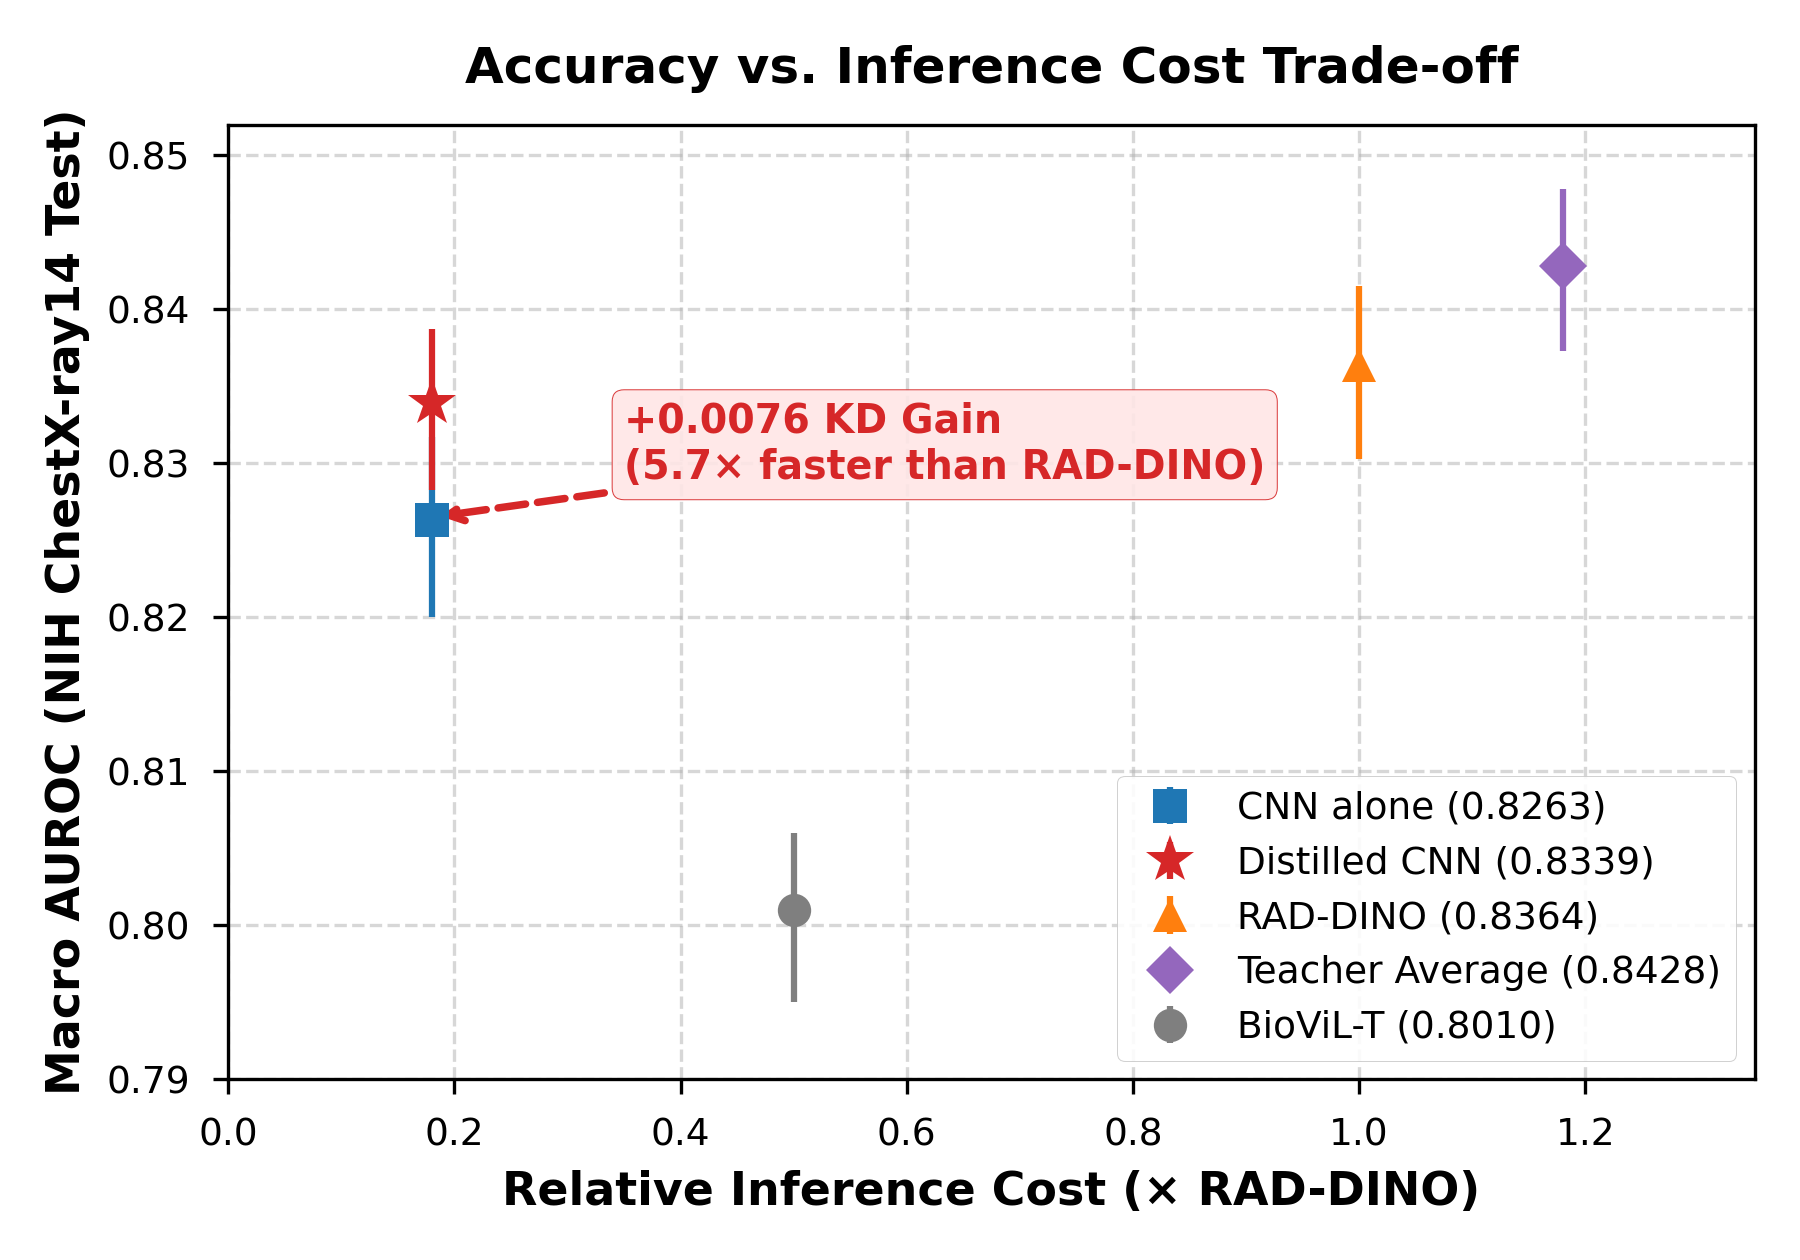
\includegraphics[width=\columnwidth]{figures/tradeoff_plot.png}
\caption{Accuracy vs.\ inference cost trade-off on NIH ChestX-ray14 test set. The Distilled CNN achieves performance close to RAD-DINO at $5.7\times$ lower compute cost ($0.18\times$).}
\label{fig:tradeoff}
\end{figure}

Relative to the CNN baseline, distillation increased macro AUROC, macro AUPRC,
macro F1, macro recall, and macro precision. As visualized in \cref{fig:tradeoff}, the gain in macro AUROC was statistically significant (+0.0076, 95\% CI +0.0058 to +0.0096, $p=0.003$), closing 75\% of the AUROC gap between the baseline CNN and RAD-DINO. Notably, the distilled student achieved a macro recall of 0.4622 (+0.0318 over baseline CNN), fully matching RAD-DINO's macro recall (0.4616). The difference in AUROC from RAD-DINO was not statistically significant ($-0.0025$, $p=0.078$). The pre-specified margin for declaring a formal match to RAD-DINO (lower CI bound $\ge -0.005$) was missed by 0.0006, so the result is reported as a significant improvement over the CNN baseline rather than equivalence to RAD-DINO.

\subsection{Paired comparisons}
\label{sec:paired-comparisons}

\Cref{tab:paired-results} summarizes the paired comparisons for the primary
metrics. The distilled model was consistently better than the CNN baseline.
Its differences from RAD-DINO were smaller and the corresponding confidence
intervals included zero. The average of the two teacher predictions remained
significantly better than the student, showing that distillation reduced the
cost of the ensemble but did not reproduce the full ensemble performance.

\begin{table}[htbp]
\caption{Paired patient-level bootstrap comparisons. Differences are reported as model A minus model B. $p$-values are Holm corrected.}
\label{tab:paired-results}
\centering
\small
\resizebox{\columnwidth}{!}{%
\begin{tabular}{llcc}
\toprule
Comparison A $-$ B & Metric & Difference (95\% CI) & Holm $p$ \\
\midrule
Distilled $-$ CNN & AUROC & $+0.0076$ ($+0.0058$ to $+0.0096$) & 0.003 \\
Distilled $-$ CNN & AUPRC & $+0.0158$ ($+0.0109$ to $+0.0210$) & 0.003 \\
Distilled $-$ CNN & Macro F1 & $+0.0163$ ($+0.0103$ to $+0.0230$) & 0.003 \\
Distilled $-$ CNN & Macro Recall & $+0.0318$ ($+0.0247$ to $+0.0389$) & 0.003 \\
Distilled $-$ CNN & Macro Prec. & $+0.0137$ ($+0.0050$ to $+0.0278$) & 0.003 \\
Distilled $-$ RAD-DINO & AUROC & $-0.0025$ ($-0.0056$ to $+0.0004$) & 0.078 \\
Distilled $-$ RAD-DINO & AUPRC & $-0.0077$ ($-0.0180$ to $+0.0010$) & 0.088 \\
Distilled $-$ RAD-DINO & Macro F1 & $-0.0086$ ($-0.0204$ to $+0.0030$) & 0.192 \\
Distilled $-$ RAD-DINO & Macro Recall & $+0.0006$ ($-0.0138$ to $+0.0165$) & 0.890 \\
Distilled $-$ teacher avg. & AUROC & $-0.0089$ ($-0.0112$ to $-0.0071$) & 0.003 \\
\bottomrule
\end{tabular}%
}
\end{table}

\textbf{Recovery of silent misses.} Out of 12,322 positive finding occurrences missed by the baseline CNN across all test images, RAD-DINO correctly identified 2,831 cases. Distillation enabled the single ConvNeXt-Tiny student to recover 1,517 of these positive findings—recovering over 53\% of RAD-DINO's detection capability on hard positives without running RAD-DINO at test time.

\textbf{Regularization against noisy labels.} Analysis of training loss dynamics showed that after its best validation epoch (epoch 6), the baseline CNN's validation loss increased from 0.305 to 0.316 due to overfitting on noisy text-mined targets. In contrast, the distilled student's validation loss remained flat (0.300 to 0.301), demonstrating that soft teacher targets ($q_{i,c} = 0.5 y_{i,c} + 0.5 q^{\text{teacher}}_{i,c}$) effectively regularize model optimization.

\subsection{Performance across findings}
\label{sec:finding-results}

The improvement was observed for all 14 findings relative to the CNN baseline,
but the magnitude varied by finding. The student was closest to RAD-DINO on
Infiltration, Consolidation, Edema, and Pneumonia. The largest remaining gaps
were observed for Pneumothorax, Pleural Thickening, and Emphysema, which are
also findings for which the higher-resolution transformer had a clearer
advantage. Hernia had the largest numerical improvement over the CNN, although
only 86 positive test cases were available.

\begin{table}[htbp]
\caption{Per-finding test AUROC. The teacher average is included to show the upper bound obtained by running both models. An asterisk ($*$) marks a finding with fewer than 100 positive test cases.}
\label{tab:per-finding}
\centering
\small
\resizebox{\columnwidth}{!}{%
\begin{tabular}{lrrrrr}
\toprule
Finding & Pos. cases & CNN & RAD-DINO & Teach. avg. & Distilled \\
\midrule
Infiltration       & 6{,}112 & 0.709 & 0.709 & 0.717 & 0.711 \\
Effusion           & 4{,}658 & 0.839 & 0.843 & 0.848 & 0.841 \\
Atelectasis        & 3{,}279 & 0.790 & 0.798 & 0.804 & 0.796 \\
Pneumothorax       & 2{,}665 & 0.882 & 0.904 & 0.905 & 0.889 \\
Consolidation      & 1{,}815 & 0.761 & 0.761 & 0.772 & 0.767 \\
Mass               & 1{,}748 & 0.846 & 0.851 & 0.860 & 0.851 \\
Nodule             & 1{,}623 & 0.798 & 0.803 & 0.817 & 0.803 \\
Pleural Thickening & 1{,}143 & 0.794 & 0.814 & 0.817 & 0.801 \\
Emphysema          & 1{,}093 & 0.936 & 0.949 & 0.948 & 0.939 \\
Cardiomegaly       & 1{,}069 & 0.888 & 0.898 & 0.904 & 0.895 \\
Edema              & 925     & 0.858 & 0.856 & 0.866 & 0.864 \\
Pneumonia          & 555     & 0.727 & 0.729 & 0.742 & 0.735 \\
Fibrosis           & 435     & 0.829 & 0.849 & 0.851 & 0.843 \\
Hernia$^{*}$       & 86      & 0.910 & 0.944 & 0.949 & 0.940 \\
\midrule
Macro average      & 27{,}206 & 0.826 & 0.836 & 0.843 & 0.834 \\
\bottomrule
\end{tabular}%
}
\end{table}

\begin{figure}[htbp]
\centering
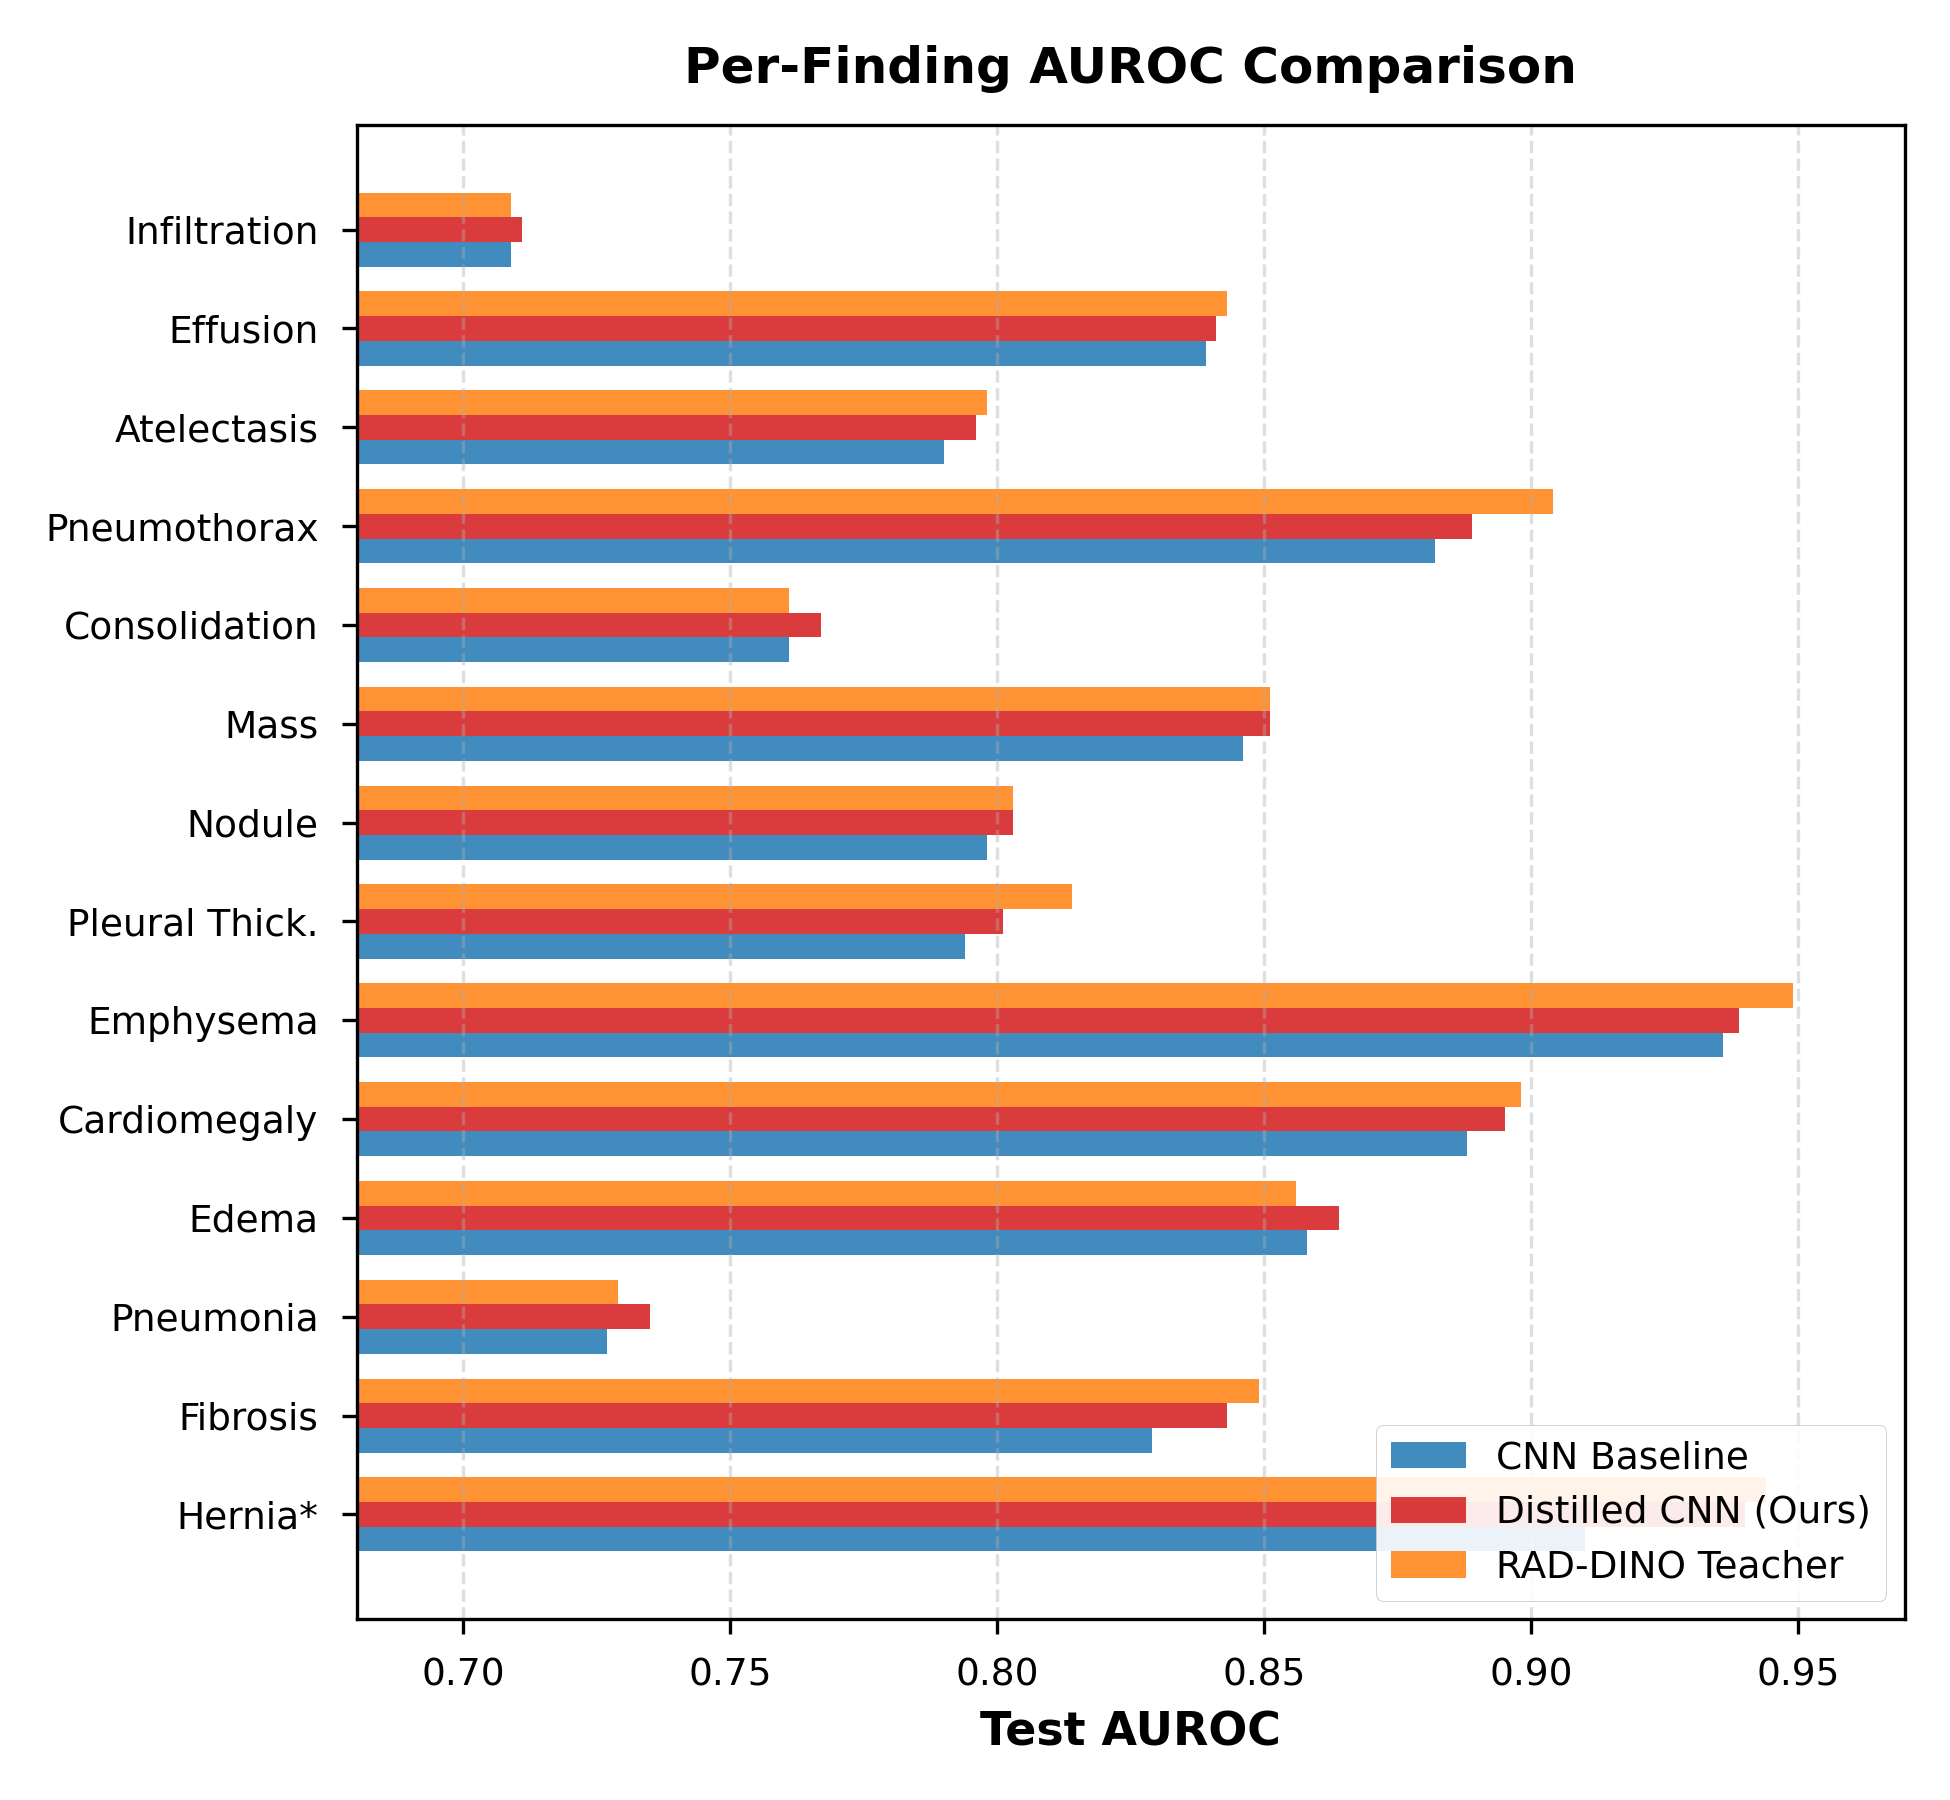
\includegraphics[width=\columnwidth]{figures/per_finding_plot.png}
\caption{Visual per-finding AUROC comparison between CNN baseline, Distilled CNN, and RAD-DINO across all 14 findings (\cref{tab:per-finding}).}
\label{fig:per-finding-bar}
\end{figure}

\subsection{Training recipe and model distillation}
\label{sec:recipe-results}

The official test results also separate the effect of the training recipe from
the effect of distillation. the training setup
provided the larger improvement, while distillation supplied an additional
gain without increasing inference cost. This comparison should therefore be
interpreted as a comparison of complete training pipelines, not as an isolated
backbone comparison.

The teacher average had a training-set macro AUROC of 0.9165 and a validation
macro AUROC of 0.8735. The pre-specified go decision was consequently met. The
student was trained using a mixture of the original labels and the teacher
probabilities. Validation performance peaked at the sixth epoch for both the
baseline and the student, and the student required approximately the same
training procedure as the baseline after the teacher probabilities had been
computed.


\begin{table}[htbp]
\caption{Main systems: accuracy and cost on the official test set. Distilled CNN matches ensemble accuracy at lower cost.}
\label{tab:cost-summary}
\centering
\small
\resizebox{\columnwidth}{!}{%
\begin{tabular}{lccc}
\toprule
System & Macro AUROC & Macro F1 & Relative cost \\
\midrule
CNN alone & 0.8263 & 0.3539 & 0.18$\times$ \\
Distilled CNN & 0.8339 & 0.3702 & 0.18$\times$ \\
RAD-DINO & 0.8364 & 0.3788 & 1.00$\times$ \\
Average of both & 0.8428 & 0.3818 & 1.18$\times$ \\
\bottomrule
\end{tabular}%
}
\end{table}



\FloatBarrier

% =====================================================================
\section{Discussion}
\label{sec:discussion}
Distillation moves the teacher ensemble's soft labels into a single small CNN, and the gains follow from what those labels contain. The teacher combines two models that make partly different errors, so its probabilities were graded rather than binary (0.28 on average for positives, 0.03 for negatives), and such soft targets reduce overfitting to noisy labels~\cite{li2017noisy}, which matters for text-mined ChestX-ray14 labels~\cite{oakdenrayner2020exploring}. Accordingly, the student's validation loss stayed flat where the CNN's rose, and it improved even on noisy, look-alike findings such as Infiltration, Consolidation and Pneumonia. Gains were largest on Mass, Atelectasis and Cardiomegaly and smaller on Emphysema, Pneumothorax and Pleural thickening, findings that depend on fine detail that RAD-DINO sees at 518\,px and the student at 384\,px; this matches the capacity-gap literature~\cite{cho2019efficacy,mirzadeh2020teacher} and points to a higher-resolution student as the next step. In practice the student needs one network, one input resolution and the compute of a small CNN, and it is significantly more accurate than the original CNN at the same cost and within 0.0025 macro AUROC of RAD-DINO at 5.7$\times$ lower batch cost, so it is the best system we tested under a limited budget, while RAD-DINO or the teacher ensemble remain preferable when compute is not constrained. This extends earlier CXR distillation work with compact students~\cite{ho2020utilizing,termritthikun2024explainable,kishore2025enhancing} to a teacher built on a CXR foundation model; we do not compare absolute AUROC with those studies, since different splits of ChestX-ray14 are not comparable and the official test split used here is harder than the development data (\cref{tab:data}). Several limitations apply: each model was trained once (seed 42), so the intervals reflect test-set sampling rather than retraining variability; the teacher includes the CNN itself, and self-distillation alone can improve a network~\cite{furlanello2018born}, so single-model teachers would be needed to separate the two effects; the labels are text-mined, the study uses one dataset, the cost figures cover the forward pass only, and the per-finding and error analyses were exploratory.

% =====================================================================
\bibliographystyle{IEEEtran}
\bibliography{references}

\end{document}

